\documentclass[fontsize=4.5pt]{scrartcl}

%
% Original Page by LinuxMercedes
%

\usepackage[
        nohead,
        nofoot,
        left=0.55in,
        right=0.55in,
        top=0.55in,
        bottom=0.55in,
]{geometry}

\usepackage{amsmath,scalefnt}

\usepackage{graphicx}
\graphicspath{ {images/} }

\renewcommand*{\arraystretch}{.5}

\usepackage{multicol}
\setlength{\columnsep}{5pt}

\usepackage{helvet}
\renewcommand{\familydefault}{\sfdefault}

\pagenumbering{gobble}

\usepackage{enumitem}
\setlist[itemize]{itemsep=-1pt, itemindent=0pt, leftmargin=*}
\setlist[enumerate]{itemsep=-2pt, itemindent=0pt, leftmargin=*}

% Commented out titlesec - incompatible with KOMA-Script
% \usepackage[compact]{titlesec}
% \titlespacing{\section}{-1pt}{-1pt}{-1pt}
% \titlespacing{\subsection}{-1pt}{-1pt}{-1pt}

\usepackage{listings}

%Y hoy yo reza que no empleo ni alma pobre encontrará esta magica negra.
%This is a custom 'tight' matrix for this cheatsheet. It's ugly.
\newenvironment{tmatrix}%
{ 
  %\scalefont{.5}
  %\setlength{\tabcolsep}{5pt}
  $\left[\hspace{-3.5pt}\begin{array}{c@{\hspace{1pt}}c@{\hspace{1pt}}c@{\hspace{1pt}}|@{\hspace{0pt}}c}
}%
{
   \end{array}\hspace{-3.5pt}\right]$
}

\newenvironment{tmatrix3}%
{ 
  %\scalefont{.5}
  %\setlength{\tabcolsep}{5pt}
  $\left[\hspace{-3.5pt}\begin{array}{c@{\hspace{1pt}}@{\hspace{1pt}}c@{\hspace{1pt}}c@{\hspace{3pt}}}
}%
{
   \end{array}\hspace{-3.5pt}\right]$
}

\newenvironment{tmatrix1}%
{ 
  $\left[\hspace{-3.5pt}\begin{array}{c@{\hspace{3pt}}}
}%
{
   \end{array}\hspace{-3.5pt}\right]$
}


\DeclareMathSizes{3pt}{3pt}{3pt}{3pt}

\begin{document}

\begin{multicols}{3}
   \section{Memory Management}
      \subsection{Requirements}
        \begin{itemize}
          \item \textbf{Relocation}: Programmer/compiler does not know where program will be in memory. Program may also be 
                    moved around during execution. Memory references in the code must be translated.
          \item \textbf{Protection}: Processes shouldn't be allowed to access other's memory without permission. Impossible to know
                    values since program can be relocated, which requires runtime checks. OS cannot anticipate all accesses of a program.
          \item \textbf{Sharing}: Allow several processes to share the same portion of memory. Better to allow each
                    process access to the same copy of a program than have separate copies.
        \end{itemize}
        \subsection{Methods - Fixed Partitioning}
        \begin{itemize}
          \item Memory is divided into partitions which are assigned on demand. These can be equal or variable-sized.
          \item Inefficient, any program, no matter how small, occupies and entire partition.  
          \item \textbf{Strategies}: Equal-sized requires no strategy. Unequal typically assigns each process to the smallest partition which it can fit,
                wasting the least amount of memory.
          \item \textbf{Partition Assignment}: Can give each partition a queue or have a main queue for the entire memory for processes to wait.
        \end{itemize}
        \subsection{Methods - Dynamic Partitioning}
        \begin{itemize}
          \item Processes are allocated exactly as much memory as required.
          \item Eventually holes start appearing in memory (unallocated bits when processes finish).
          \item \textbf{External Fragmentation}: Chunks of unallocated memory left from processes finishing. When all over, processes can't find space.
          \item \textbf{Internal Fragmentation}: With fixed page sizes, the last page of a program that can be partially filled.
          \item Must use \textbf{compaction} to shift processes so they are contiguous and free memory is in one block.
        \end{itemize}
        \subsection{Strategies for Dynamic Partitioning}
        \begin{itemize}
          \item \textbf{First-fit}: fastest, however can have many processes allocated at front end that must be searched over
                while searching for a new block. Looks for the first block of memory that fit.
          \item \textbf{Best-fit}: Worst performer, chooses block that is closest in size to request. Causes more computation to be
                required as external fragments are the smallest too.
          \item \textbf{Next-fit}: Like first fit, but searches for free blocks beyond the last (time) allocated block. Results in event distribution of free block
                in memory.
        \end{itemize}
        \subsection{Methods - Buddy System}
        \begin{itemize}
          \item Entire space is treated as a single block of $2^{u}$. If a request of size s is such that $2^{u-1}<s\leq2^{u}$ then
          the entire block of $2^{u}$ is allocated.
          \item Otherwise, split into two equal buddies.
          \item Splitting continues until smallest block $\geq$ s is generated.
          \item Data structure resembles a binary tree.
          % If this is on the test, slide 10 of chap7 has an example that looks decent...
          % http://i.brod.es/dpaEb.png
         \end{itemize}
    
    \section{Virtual Memory}
      % I'm skipping tons of stuff I _know_ here because of homework 2
      \begin{itemize}
       \item \textbf{Page Fault}: Page table indicates that virtual address isn't in memory, os exception handler is invoked to move data from disk to memory.
       \item \textbf{Translation Lookaside Buffer}: High speed cache to look up page table entries. Stores most recently used page table entries. Uses associative mapping (many page
              numbers can map to the same TLB index).
       \begin{itemize}
          \item Given a virtual address, the processor examines the TLB.
          \item If a page table entry is present, it's a ``hit'' and the frame number is returned which leads to the read address.
          \item If it isn't (``miss''), the page number is used to look it up, and the TLB is updated with this data.
       \end{itemize}
       % Optional diagram for how this works Slide 20 Chap8-1
      \end{itemize}
      \subsection{Page Sizes}
      \begin{itemize}
       \item Multi-level page tables allow for a new page table above another, which then maps to other entries. 
       \item Smaller page side leads to less internal fragmentation, larger page tables, and page tables ending up in virtual memory (as they are so large). This can, in turn, lead to double page faults.
       \item Small page sizes means more pages fit in memory, leading to fewer page faults. This is due in part to smaller pages that are used frequently staying in memory, instead of large chunks with a small bit
             used taking up space.
       \item Secondary memory is designed to transfer large chunks of data efficiently, which favors large page sizes.
       \item Larger page sizes leads to some useless references being in memory taking up space.
      \end{itemize}
      % Paging algorithms, including OPT which requires prior knowledge for it to work... keeps pages in memory just right
  \section{Uniprocessor Scheduling}
    \subsection{Aims}
      \begin{itemize}
       \item \textbf{Response Time}: time it takes a system to reactive to a given input (reduce).
       \item \textbf{Turnaround time}: (TAT) total time spent in the system, waiting time + service time.
       \item \textbf{Throughput}: jobs per minute (inverse of TAT), maximize.
      \end{itemize}
      \subsection{Types}
      \begin{itemize}
       \item \textbf{Long-Term Scheduling}
       \begin{itemize}
         \item Determines which programs are admitted to system for processing
         \item Controls degree of multiprogramming
         \item Which job to admit? FCFS, Priority, expected exec time, I/O reqs
       \end{itemize}
       \item \textbf{Medium-Term Scheduling}
       \begin{itemize}
         \item Part of the swapping function
         \item Swapping-in decision is based on the need to manage the degree of multiprogramming
       \end{itemize}
       \item \textbf{Short-term scheduling} is the \textbf{dispatcher}. It executes most frequently and is invoked when events occur. Including clock interrupts, I/O, OS calls, signals, etc.
      \end{itemize}
      \subsection{Factors}
        \begin{itemize}
        \item Priorities: scheduler should choose higher priority processes over lower priority ones. Uses many ready queues to represent each level. Lower priority processes can suffer starvation.
        \item Decision Modes:
          \begin{itemize}
            \item \textbf{Nonpreemptive}: Once a process is in the running state, it will continue until termination or blocks self.
            \item \textbf{Preemptive}: Currently running process can be interrupted and moved to the ready state due to external event. No single process can monopolize processor for long.
          \end{itemize}
        \end{itemize}
      \subsection{Schedulers}
        \begin{itemize}
         \item First-Come-First-Serve (FCFS): nonpreemptive scheduler where oldest process is scheduled to run next.
         \begin{itemize}
           \item Advantage: favors CPU-bound processes. I/O processes wait for CPU bound ones to finish.
           \item Disadvantage: Short processes can wait for a long time before running.
         \end{itemize}
         \item Round Robin (RR): preemptive based on clock (time sliced) interrupt at regular intervals. When an interrupt occurs, process is placed into ready and next job runs.
         \item Shortest Process Next (SPN): Nonpreemptive, process with shortest \textbf{expected} processing time is next. For batch jobs, user is required to estimate the running time
               . For interactive jobs, OS predicts it. Short processes get priority here and long ones can be starved.
         \item Shortest Remaining Time (SRT): Preemptive version of $\wedge$. Achieves better turnaround time to $\wedge$ as a short job is given immediate preference to a long one. Hard to estimate remaining time.
         \item Highest Response Ratio Next (HRRN): Nonpreemptive, uses R= (time spent waiting + service time ) / service time decide next process. No starvation possible, shorter jobs preferred.
        \end{itemize}
  \section{Multiprocessing}
    \subsection{Issues}
      \begin{itemize}
        \item Multiprogramming usage--- should we allow one application to lock up several cores (maximum speedup)?
        \item Unless a single queue is used for scheduling, it becomes more difficult to maintain specific disciplines.
        \item When a single queue is used, a single process can be schedule to run on any processor (master node needed).
        \item Preemptive schemes (RR) are costly to implement with a single queue approach.
      \end{itemize}
     \subsection{Real-time systems}
       \begin{itemize}
         \item Tasks or processes attempt to control/react to events which must keep up.
         \item Correctness depends on both result AND time at delivery.
         \item Critical that the system is reliable, sometimes with failsafe (traffic lights).
         \item Sometimes include small size, fast context switches, prioritization of scheduling, and special alarms/timeouts.
         \item \textbf{Hard real-time task}: must meet the deadline, causes catastrophic failure/errors w/o.
         \item \textbf{Soft real-time task}: has a deadline that is desired. Makes sense to complete even if late.
         \item \textbf{Periodic tasks}: Only one unit per period T, exactly T apart.
         \item \textbf{Aperiodic task}: has a deadline by which it must finish/start/both.
       \end{itemize}
      \subsection{Deadline scheduling}
        \begin{itemize}
          \item Real time application, not concerned with fairness/response time but with prioritizing tasks based on deadlines.
          \item Earliest deadlines typically scheduled first.
          % there's 2 example slides here, slide 13/14 on chap10.
          \item Best to know each first:
          \begin{itemize}
            \item Ready time (periodic tasks know this)
            \item Starting/completion deadline
            \item Processing time and resource reqs.
            \item Priority
           \end{itemize}
        \end{itemize}
      \subsection{Rate Monotonic Scheduling}
        \begin{itemize}
          \item Assigns priorities to tasks on basis of periods.
          \item Highest priority tasks have the shortest period.
          \item Always works if the below is satisfied:\\
          $\frac{C_1}{T_1} + \frac{C_2}{T_2} + \dots + \frac{C_n}{T_n} \le n(2^{\frac{1}{n}}-1)$
          \item Has industrial applications.
          \item Higher priority tasks have higher frequencies (hz)
          \item n is the number of tasks, C is cycle time T is processing time?
        \end{itemize}
        % Unix SVR scheduling skipped
  \section{Networking}
    \subsection{Internet Protocol}
      \begin{itemize}
        \item Uniform method for host addresses, each host getting a unique one.
        \item Provides packet delivery mechanisms (\textbf{Packet}: standard transfer unit), packets having a header with destination and size and a payload.
        \item ISO Open Systems Interconnect Model has 7 layers. From top to bottom: Application, presentation, session, transport, network, data link, physical.
        \item ISO OSI is a framework for specific protocols (FTP/RPC/TCP).
      \end{itemize}
     \subsection{Low Level Protocols}
       \begin{itemize}
         \item Physical layer is the signaling tech--- all hardware.
         \item Data link layer, frame management. MAC addresses, form of hexadecimal letters X XX:XX:XX:XX:XX:XX, 6 pairs.
         \item Broadcasts are on 6 pairs of FF.
         \item Examples are wireless, Ethernet, and X.25.
         \item These addresses are 48 bit.
         \item Hosts send bits to other hosts in \textbf{frames}.
         \item Hubs take one frame and send it to every other port.
       \end{itemize}
     \subsection{OSI Layers (cont)}
       \begin{itemize}
         \item Network layer
         \begin{itemize}
           \item Combines networks using IP. 
           \item Performs packet routing across \textbf{gateways}, intermediate hosts.
         \end{itemize}
         \item Transport Layer
         \begin{itemize}
           \item TCP makes conns. on network w/ sockets, using IP/ports.
           \item Keeps track of order of packet delivery.
           \item Ensures all data arrives at destination in order (ACK/SYN).
           \item Two basic protocols: TCP and UDP.
           \item TCP is transmission control protocol, which is stream-oriented. Unduplicated and reliable.
           \item UDP is user datagram protocol which gives no guarantee of delivery or duplication. (more efficient)
           % graphic on header structure. TCP has tons of stuff including what sort of packet (ACK/SYN/etc) while UDP has a payload, checksum, and dest/port.
         \end{itemize}
          \item Presentation Layer: converts local representations of data into its canonical form.
          \item Application layer: provides network services to end users, FTP clients, telnet, SMTP.
        \end{itemize}
     \subsection{Domain Name System}
       \begin{itemize}
         \item Translates symbolic hostnames into IP addresses
         \item Hierarchical, distributed naming system for things on the internet
         \item IP uses 32-bit address (4 sets of \#s, 0-255)
         \item Each (sub)domain has 1+ \textbf{authoratative} DNS servers that public info to name servers.
         \item DNS server maintains list of resolutions.
       \end{itemize}
      
      \subsection{Sockets}
        \begin{itemize}
          \item BSD sockets enable communication between client/server.
          \item Semantics resemble pipes (files), bidirectional.
          \item Once one is created it can be bound to a port.
          \item A server assigns an address to its socket + tells all potential clients.
          \item Servers are passive and always waiting for clients to do something.
          \item A client obtains correct socket address of any server.
          \item Clients are active and run automatically deciding when to use a server.
          \item Low level ports reserved for OS.
          \item Each port can be bound to an address and used by an application.
        \end{itemize}
  \section{Distributed Processing}
    \subsection{Applications}
      \begin{itemize}
        \item \textbf{Databases}:
        \begin{itemize}
          \item Databases is a very common family of distrib. proc w/ client/servers.
          \item The server in a database maintains it
          \item Clients use transactions to interact, usually over IP. Many clients can coexist.
        \end{itemize}
        \item Thinclients (dumb terminals / VM)
        \item \textbf{Three tier models}:
        \begin{itemize}
          \item Application software distributed on all 3.
          \item Users use a thin client, while the backend has ``legacy applications''
          \item Middle tier has gateway, protocol conversion, mapping, and is both a client and a server
        \end{itemize}
      \end{itemize}
     \subsection{Issues}
       \begin{itemize}
         \item Lack of standards leads to \textbf{middleware}.
         \begin{itemize}
           \item Sets of tools to provide uniform style of access and usage across a platform.
           \item Provides standard programming interfaces/protocols to sit in the middle of client/servers.
           \item Handles complexities and disparities.
           \item \textbf{SOA}, service oriented architecture. Services with well defined interfaces are given to other groups to maintain.
           \item XML via HTTP is a popular interface for communication between services.
           \item RPC is another standard (remote procedure calls).
         \end{itemize}
         \item Message passing schemes
         \begin{itemize}
           \item Guarantees delivery if possible
           \item Send the message out without reporting failure/success reduces overhead and allows queueing.
           \item Blocking: send does not return control to sending process until sent, does not return control until ACK'd, or not returned until buffered for send.
           \item Nonblocking: process is not suspended as result of send/received, difficult to debug but efficient.
         \end{itemize}
       \end{itemize}
      \subsection{Clusters}
        \begin{itemize}
          \item Alternative to SMP--- group of interconnected comps working as unified source, acts as once machine.
          \item SMP is easier to manage and configure.
          \item SMP takes up less space, uses less power.
          \item Clusters are better for incremental / abs scalability
          \item $\wedge$ superior in terms of availability
          \item $\wedge$ Better price/performance.
          \item Load balancing is a problem for clusters.
          \item Failure management is another issue--- failure tolerant or highly available?
        \end{itemize}


  \section{Glossary}
    \subsection{Exam 1}
      \begin{itemize}
        \item \textbf{Address Translator} – A functional unit that transforms virtual addresses to real addresses
        \item \textbf{Busy waiting} – the repeated execution of a loop of code while waiting for an event to occur
        \item \textbf{Context Switch} – an operation that switches the processor from one process to another, by saving all the process control block, registers, and other information for the first and 
                                        replacing them with the process information for the second
        \item \textbf{Direct Memory Access (DMA)} – a form of I/O in which a special module, called a DMA module, controls the exchange of data between main memory and an I/O device.  
                                    The processor sends a request for the transfer block of data to the DMA module and is interrupted only after the entire block has been transferred.
        \item \textbf{File Allocation Table (FAT)} – a table that indicates the physical location on secondary storage of the space allocated to a file.  There is one file allocation table for each file.
        \item \textbf{Job Control language (JCL)} – a problem-oriented language that is designed to express statements in a job that are used to identify the job or to describe its requirements to an operating system
        \item \textbf{Kernel} – a portion of the operating system that includes the most heavily used portions of software.  Generally, the kernel is maintained permanently in main memory.  
                The kernel runs in a privileged mode and responds to calls from processes and interrupts from devices.
        \item \textbf{Race Condition} – an undesirable situation that occurs when a device or system attempts to perform two or more operations at the same time, but because of the nature of the device or system, 
        the operations must be done in the proper sequence in order to be done correctly.
        \item \textbf{Starvation}: process is delayed forever as other processes are always given preference.
        \item \textbf{Time Sharing} – the concurrent use of a device by a number of users
        \item \textbf{Time Slicing} – a mode of operation in which two or more processes are assigned quanta of time on the same processor
      \end{itemize}
    \subsection{Exam 2}
      \begin{itemize}
         \item \textbf{Base Address}: an address that is used as the origin in the calculation of addresses in the execution of a computer program.
         \item \textbf{Dynamic Relocation}: a process that assigns new absolute addresses to a computer program during execution so that the program may be executed from a different area of main storage.
         \item \textbf{Indexed Sequential Access}: pertaining to the organization and accessing of the records of a storage structure through an index of the keys that are stored in arbitrarily partitioned sequential files.
         \item \textbf{Logical Address}: a reference to a memory location independent of the current assignment of data to memory.  A translation must be made to a physical address before the memory access can be achieved.
         \item \textbf{Page}: in virtual storage, a fixed length block that has a virtual address and that is transferred as a unit between main memory and secondary memory.
         \item \textbf{Paging}: the transfer of pages between main memory and secondary memory.
         \item \textbf{Physical Address}: the absolute location of a unit of data in memory (e.g., word or byte in main memory, block on secondary memory).
         \item \textbf{Sequential Access}: the capability to enter data into a storage device or a data medium in the same sequence as the data are ordered or to obtain data in the same order as they were entered.
         \item \textbf{Sequential File}: a file in which records are ordered according to the values of one or more key fields and processed in the same sequence from the beginning of the file.
         \item \textbf{Spooling}: the use of secondary memory as buffer storage to reduce processing delays when transferring data between peripheral equipment and the processors of a computer.
         \item \textbf{Trojan Horse}: secret undocumented routine embedded within a useful program.  Execution of the program results in execution of the secret routine.
         \item \textbf{Virtual Address}: the address of a storage location in virtual storage.
      \end{itemize}
    
    
  \section{QA Pool}
    \subsection{Memory Management}
      \begin{itemize}
        \item \textbf{Page fault trap} interrupt is created when a desired page frame isn't in RAM.
        \item \textbf{Valid bit} is set in the page table when it is not in RAM. This is how it knows it isn't.
        \item \textbf{Dirty bit}s are set when a page frame has been modified.
        \item \textbf{Locality}: process executes in clustered pages (low fragmentation). Bad is opposite.
        \item \textbf{Global allocation}: allows a proc. to select a replacement frame from a set of all frames, even if it's given to some other process; processes can steal frames.
        \item \textbf{Working set allocation}: assumes processes execute in localities. Each process should be alloc'd enough frames for current set.
        \item Which of the two above are more affected by bad locality? Working set as those with bad locality have poorly defined working sets, so more page faults.
        \item Page fault timeline:
        \begin{itemize}
          \item OS blocks proc, puts in waiting queue
          \item Ready queue proc. is selected to run
          \item DMA is initiated to load faulted page
          \item Page replacement strat. ran
          \item Page table updated to reflect change
        \end{itemize}
        \item TRUE: When a DMA takes place, processor does other things.
        \item FALSE: DMA interrupts CPU by stealing cycles.
        \item Largest program that can execute on a comp. with 24-bit virtual addresses is a $2^{24}$ byte program.
        \item Same question as $\wedge$ but with hardware: can't tell, need to know virt. size.
        \item Address in a \textbf{TLB} entry \textbf{PTE} is physical.
        \item Flags in a PTE: valid bit, reference bit, dirty bit.
        \item \textbf{Hit-ratio}: in 2 level memory system (RAM-HD/cache-RAM), it is the frac of mem accesses found in master (first).
        \item FALSE: Misses in the \textbf{TLB} guarantee entries in the page table entry--- \textit{X may not be resident in RAM}.
        \item TRUE: It is possible that page tables are stored in virtual memory.
        \item TRUE: page sizes must be large enough to offset high cost of page faults.
        \item TRUE: in virt. mem. system, cannot run program whose size $>$ main mem.
%         \item \textbf{Diagram for relationship between virtual memory components}: There will be 6 boxes, Virtual Address, TLB (full name above), Page Table, Real Address, 
%               Main Memory, and Secondary memory. This is read from left to right, TLB is above Page Table and Real Address is to the right of Page Table. Main memory is then next
%               with secondar memory to the right of that. An arrow for page fault spans the bottom of the diagram, from the first box (Virt Address) to Secondary Memory.
%         \begin{itemize}
%           \item First unit is a virtual address box with two sections, page \# and offset.
%           \item Page \# has three arrows coming from it, the first arrow is labeled ``page fault'' and goes to a block
%                 on a secondary memory column.
%           \item The block on the secondary memory column then goes to a block on main memory, the arrow is labeled ``load page''.
%           \item The second arrow on the first box for page \# goes to a sliver of a ``Page Table'' column where the transition is labeled ``TLB Miss''.
%           \item The sliver then goes to Real Address which, like Page Table, is a 2 part box with Frame \# and offset.
%           \item Offset then points to the same segment as load page does above in main memory, but with an ``offset''
%                 to a certain part of it (the middle here).
%           \item ``Page \#'''s final entry in Virtual Address goes to the TLB (see mem management sec at top). It splits into
%                 8 arrows and one segment is highlighted.
%           \item This one segment, called TLB hit, goes to frame \# on Real Address like TLB miss on the page table did (last bit).
%           \item The final transition is the offset for the Virtual Address. It goes directly to offset in physical address with no label.
%         \end{itemize}
        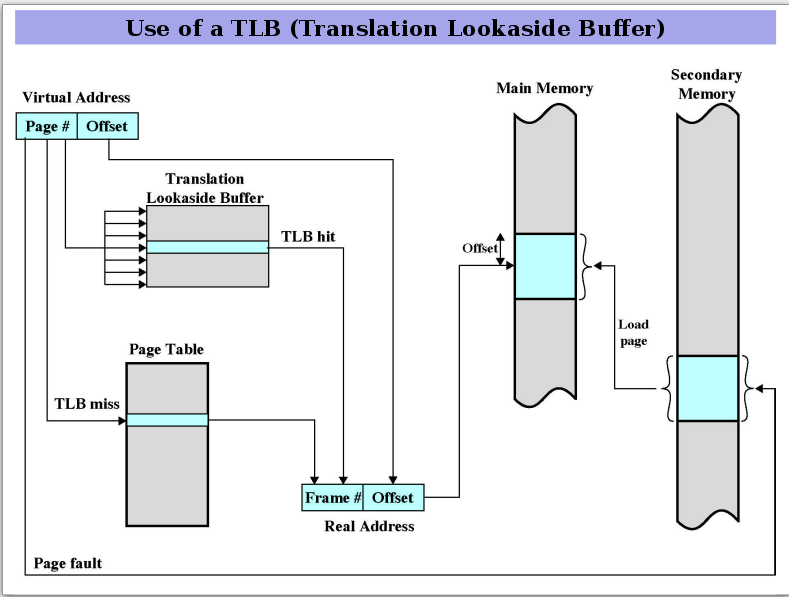
\includegraphics[scale=0.20]{virtmemuse}
        
        \item Valid bit states whether the page table entry has the disk address.
        \item \textbf{Demand Paging}: only load virtual pages as accessed.
        \item \textbf{Prepaging}: bring more pages in than needed, ones that follow.
      \end{itemize}

    \subsection{Sockets}
      \begin{itemize}
        %Several stupid questions at the beginning skipped
        \item The second argument to listen(sock,\#) determines wait queue size, not max.
        \item Fat client models DO take advantage of desktop power (they ARE desktops).
        \item All of the following socket commands descriptors return -1 on failure.
        \item socket( ..., SOCKET\_STREAM, 0 ). Creates TCP socket and rets. descriptor.
        \item bind( sd, -struct cast madness-, len ). Binds the definition of a socket to a port \#.
        \item socket( ..., SOCKET\_SOCK\_DGRAM, 0 ). Creates a UDP socket and rets. descriptor.
        \item accept( sd, -cast madness-, len ). Blocks until client connection received, returns descriptor when it happens.
      \end{itemize}
    
    \subsection{Scheduling and Processing}
      \begin{itemize}
        \item Direct goals of proc. schedulers: improve response time, throughput, TAT, efficiency
      \end{itemize}

    
    
    \subsection{Security and Triumph of the Nerds}
      \begin{itemize}
        \item Most antivirus software uses emulation / heuristics.
        \item Logic bombs, trojan horses, and viruses require a host program to operate.
        \item ``Bots'' attack require: attack software, many vulnerable machines, and locating those machines.
        \item Dennis Richie and Ken Thompson basically made C/Unix. \textbf{Worship them}.
        \item Bill Gates and Paul Allen started MS in 1975.
        \item Xerox/PARC made drop down menus, the mouse, windows, etc.
        \item Steve Jobs and Steve Wozniac co-founded Apple. The former then started NeXT and was the CEO of pixar.
        \item MSDOS was mostly QDOS, which Tim Patterson wrote, owned by CL Computer Productions, cloned by CPM, which was written by Gary Kildall.
        \item Jobs saw a GUI at PARC that inspired him to computer real good.
        \item $\wedge$ also saw OOP and e-mail which he ignored
        \item $\wedge$ created Lisa after $\wedge$ which flopped. Then created Macintosh (2nd).
        \item BASIC language interpreter kickstarted MS into the microcomp. bidness.
        \item MS got into the OS market when Kildall didn't persue IBM when they wanted a new OS. His wife/attourny didn't want to sign an NDA. Gates saw this and jumped in.
        \item Apple purchased NeXT and its OS NExTStep in 1996.
        \item \textbf{Killer App}: something so useful people buy comps to run it.
        \item Apple II's $\wedge$ was Visicalc.
        \item IBM's PC's $\wedge$ was Lotus 1-2-3.
        \item Macintosh's $\wedge$ was a WYSIWYG desktop publisher.
        \item IBM didn't create their own OS on their first PC as they wanted to make it super fast, under a year. They couldn't design much, just had to slap it together.
        \item Compaq had to reverse engineer ROM-BIOS from IBM's first PC as it was proprietary.
        \item IBM decided on an open architecture to save time. They bought computer components off the shelf and assembled them, hence ``open architecture''. As a result IBM
              also had to buy the OS and other software from other vendors.
        \item Ed Roberts at MITS built the first commercially available PC in 1975.
        \item Gordon Moore is an Intel founder.
        \item Altair 8800 was the world's first personal computer and was designed by Ed Roberts in 1975.
        \item First mass market PC company is Apple.
      \end{itemize}
     
     
     \subsection{Weird Questions}
       \begin{itemize}
         \item RAID \#'s: 1, mirror; 0, merge drives (splits data even); 10|2, striping, error detection, and fault tolerance (common).
       \end{itemize}




  \end{multicols}
\end{document}

